\section{Hasil dan Pembahasan}
\label{sec:hasildanpembahasan}

Dilakukan pengujian dan analisis terhadap perancangan dan implementasi yang telah di desain sebelumnya. Pengujian yang dilakukan meliputi pengujian Sensor Load Cell terhadap Robot dan Sistem Keseimbangan Robot. 

\begin{enumerate}[label=\Alph*.]

    \item Pengujian Karakterisasi Pada Masing-Masing Sensor Load Cell
    \label{subsec:hasil-pembahasan-karakterisasi}

        \hspace*{1em} Pengujian kalibrasi sensor load cell dilakukan dengan menggunakan lima bandul referensi massa (50g, 100g, 200g, 500g, dan 1000g) untuk menentukan koefisien gradien dan konstanta tare weight. Load cell dihubungkan dalam dua kelompok: Load Cell 1 dan 4, serta Load Cell 2 dan 3. 

        \begin{table}[h]
            \centering
            \caption{Hasil Karakterisasi Load Cell Pertama}
            \begin{tabular}{|c|c|c|}
                \hline
                \textbf{Berat Aktual (gr)} & \textbf{Load Cell 1 Pembacaan (gr)} & \textbf{Error (gr)} \\
                \hline
                50    & 50    & 0   \\
                100   & 101   & 1   \\
                200   & 202   & 2   \\
                500   & 505   & 5   \\
                1000  & 1004  & 4   \\
                \hline
            \end{tabular}
            \label{tab:Kalibrasi_Load_Cell_1}
        \end{table}
        
        \hspace*{1em} Data pembacaan digital dari load cell dihitung menjadi massa aktual menggunakan persamaan kalibrasi, dan kesalahan diukur dengan membandingkan hasil dengan massa aktual. Hasil pengukuran menunjukkan kesalahan bervariasi antara 0-3\% untuk masing-masing load cell, dan 0-2.5\% untuk load cell yang terhubung. Meskipun tidak sepenuhnya linear, persamaan kalibrasi yang digunakan cukup akurat dengan toleransi kesalahan sebesar 5\%.

    \item Pengujian Tekanan Pada Telapak Kaki
    \label{subsec:hasil-pembahasan-tekanan}

        \hspace*{1em} Pengujian ini dilakukan untuk mendapatkan data tekanan yang dihasilkan oleh kaki kanan dan kaki kiri ketika diberikan beban secara merata. Data tekanan yang dihasilkan oleh kaki kanan dan kaki kiri dapat dilihat pada Tabel \ref{tab:pengukuran_berat_kaki}.

        \begin{table}[h!]
            \centering
            \caption{Tabel Pembacaan Tekanan untuk Kaki Kiri}
            \begin{tabular}{|c|c|c|}
                \hline
                \textbf{Berat Aktual (gr)} & \textbf{Pembacaan (gr)} & \textbf{Error (gr)} \\
                \hline
                50    & 52    & 2   \\
                100   & 110   & 10  \\
                200   & 220   & 20  \\
                300   & 304   & 4   \\
                500   & 512   & 12  \\
                700   & 701   & 1   \\
                1000  & 1050  & 50  \\
                1300  & 1325  & 25  \\
                1500  & 1512  & 12  \\
                1800  & 1788  & 12  \\
                \hline
                \textbf{Rata-rata Error (gr)} & \multicolumn{2}{c|}{\textbf{14.8}} \\
                \hline
            \end{tabular}
            \label{tab:pengukuran_berat_kaki}
        \end{table}

        \hspace*{1em} Berdasarkan hasil pengujian, rata-rata kesalahan yang dihasilkan oleh kaki kiri adalah 14.8 gram. Hal ini disebabkan oleh sifar non-linearitas dari desain sistem load cell yang digunakan.

    \item Pengujian Pusat Tekanan Terhadap Robot
    \label{subsec:hasil-pembahasan-pusat-tekanan}

        \hspace*{1em} Pengujian ini dilakukan dengan menggerakkan robot dalam pola berjalan dan mengambil data input dari sensor tekanan dengan interval 120 ms. Untuk melakukan pengujian, robot diprogram untuk berjalan dengan pola gerakan tertentu. Data pusat tekanan diambil dari sensor load cell yang terpasang pada telapak kaki robot. Data yang diambil kemudian diolah untuk mendapatkan posisi pusat tekanan pada sumbu x dan y.

        \begin{figure}[h!]
            \centering
            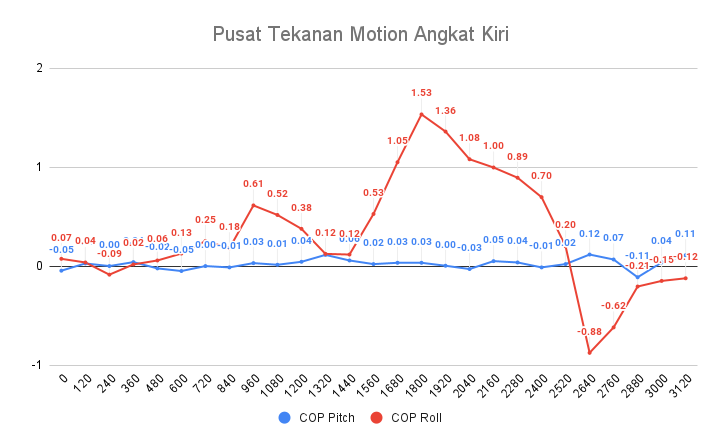
\includegraphics[width=0.45\textwidth]{gambar/Angkat_Kiri.png}
            \caption{Grafik Pusat Tekanan Ketika Robot Mengangkat Kaki Kiri}
            \label{fig:pusat_tekanan_kiri}
        \end{figure}

        \hspace*{1em} Hasil pengujian menunjukkan bahwa pusat tekanan berubah secara dinamis selama robot melakukan gerakan berjalan. Ketika robot mengangkat kaki kiri, pusat tekanan berpindah ke kaki kanan, dan nilai pusat tekan pada sumbu X memiliki nilai minimum sebesar -0.5. Pada sumbu Y, nilai pusat tekanan berada pada rentang -1 hingga 1, yang menunjukkan bahwa pusat tekanan berada di tengah-tengah telapak kaki.
\end{enumerate}